\section{Results}
\label{sec-results}

We began by randomly sampling 1000 bugs from both Linux and Firefox
and determined the types of changes, the results are shown in Table
\ref{tbl-changes}. Overall the percentages are similar for both
software projects except for when there are no changes and changes
which are only modifications. We believe this is because most of the
bugs only applied to JavaScript for Firefox which we did not analyze,
and they contain the class of bugs which are fixed by simple
modifications.

\begin{table}
\begin{center}
\begin{tabular}{l|r|r}
\multicolumn{1}{c}{} & \multicolumn{2}{c}{\textbf{Amount (\%)}} \\
\textbf{Type of Change} & \multicolumn{1}{c|}{\textbf{Linux}} & \multicolumn{1}{c}{\textbf{Firefox}}\\
\hline
None          &  7.7 $\pm$ 1.65 & 43.0 $\pm$ 3.07\\
\hline
Add           & 11.0 $\pm$ 1.94 & 6.9 $\pm$ 1.57\\
\hline
Remove        &  2.0 $\pm$ 0.87 & 1.8 $\pm$ 0.82\\
\hline
Modify        & 35.7 $\pm$ 2.97 & 13.8 $\pm$ 2.14\\
\hline
Add/Modify    & 14.9 $\pm$ 2.20 & 11.6 $\pm$ 1.98\\
\hline
Add/Remove    &  5.8 $\pm$ 1.45 & 2.3 $\pm$ 0.93\\
\hline
Modify/Remove &  5.9 $\pm$ 1.46 & 3.2 $\pm$ 1.09 \\
\hline
All           & 17.0 $\pm$ 2.33 & 17.4 $\pm$ 2.35\\
\end{tabular}
\end{center}
\caption{The types of changes between bug introductions and fixes from random sampling}
\label{tbl-changes}
\end{table}

We also noted that approximately 7.7\% of the bug fixes for Linux were
purely for comments, indicating that developers spend a non-trivial
amount of time on comments. For Linux approximately 51\% of the
changes do not include additions. We manually checked the 49\% more
difficult cases to evaluate the effectiveness of our technique.

For Linux we manually checked a random sample of 50 bugs with the
following types: 11 additions, 16 additions and modifications, 6 additions
and removals, and 17 with all types of changes. We found 10 of the 50
to be false positives. Similarly for Firefox we randomly sampled 50
bugs with the following types: 9 additions, 3 additions and
modifications, 18 additions and removals, and 20 with all types of
changes. We found 13 of the 50 to be false positives.

The are five main sources of false positives we found, first we cover
the rare cases. For one, the commit message we determined as a fix
actually referred to fixing a merge conflict. Next, the blamed author
was not correct due to them being the original author of the code, not
the one who missed a check added at a later time. Finally a removal of
dead code would trigger a non-existent bug. The more common cases
involved reverting a change so it could be added in a later version
and a code clean-up which involved moving functions or
renaming. However in some cases you could argue that some of the code
clean-ups should be counted as a bug.

Our false positive rates are currently between 20\%-26\% for the
difficult cases of bug fixes. Since these account for approximately
half of the overall fixes, we believe this is an upper bound on our
false positive rate. Taking this into account we believe our data is
representative and the results that we obtained are valid and meaningful.

\begin{figure*}
\begin{center}
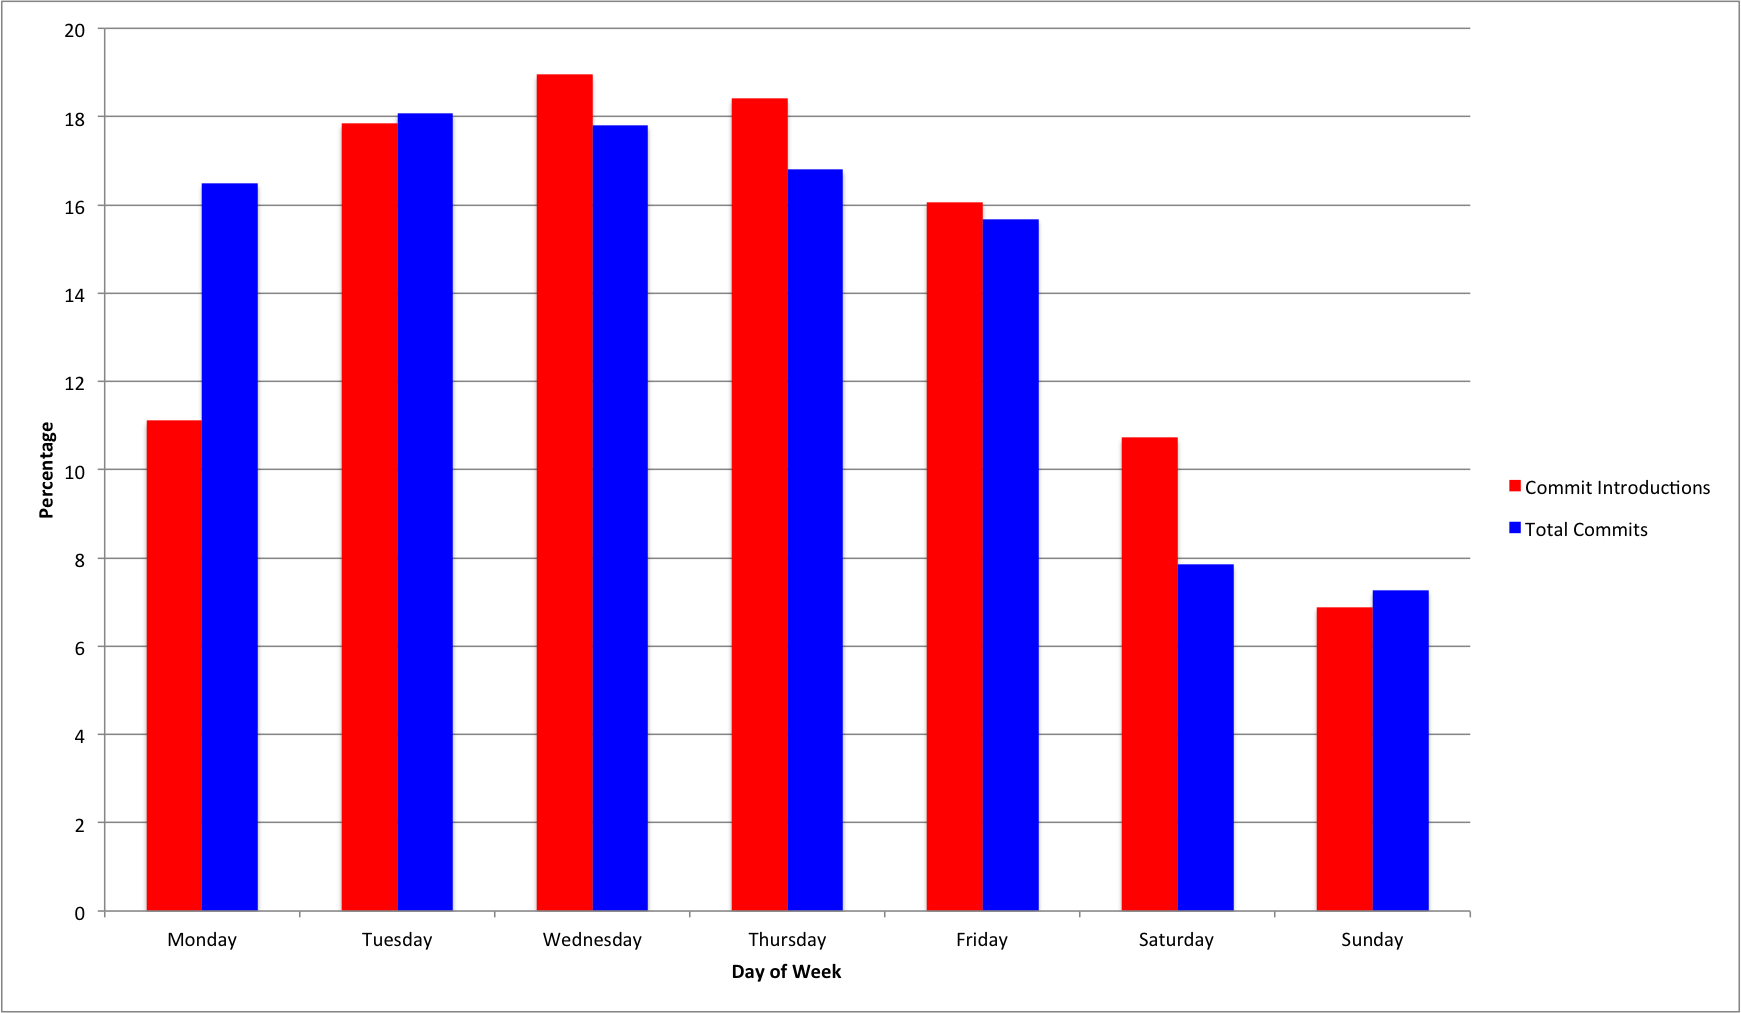
\includegraphics[width=0.9\textwidth]{linux_bug_introduction_day_of_week.png}
\end{center}
\caption{Linux percentage of bug introductions and percentage of total commits per day}
\label{fig-linux-weekday}
\end{figure*}

\begin{figure*}
\begin{center}
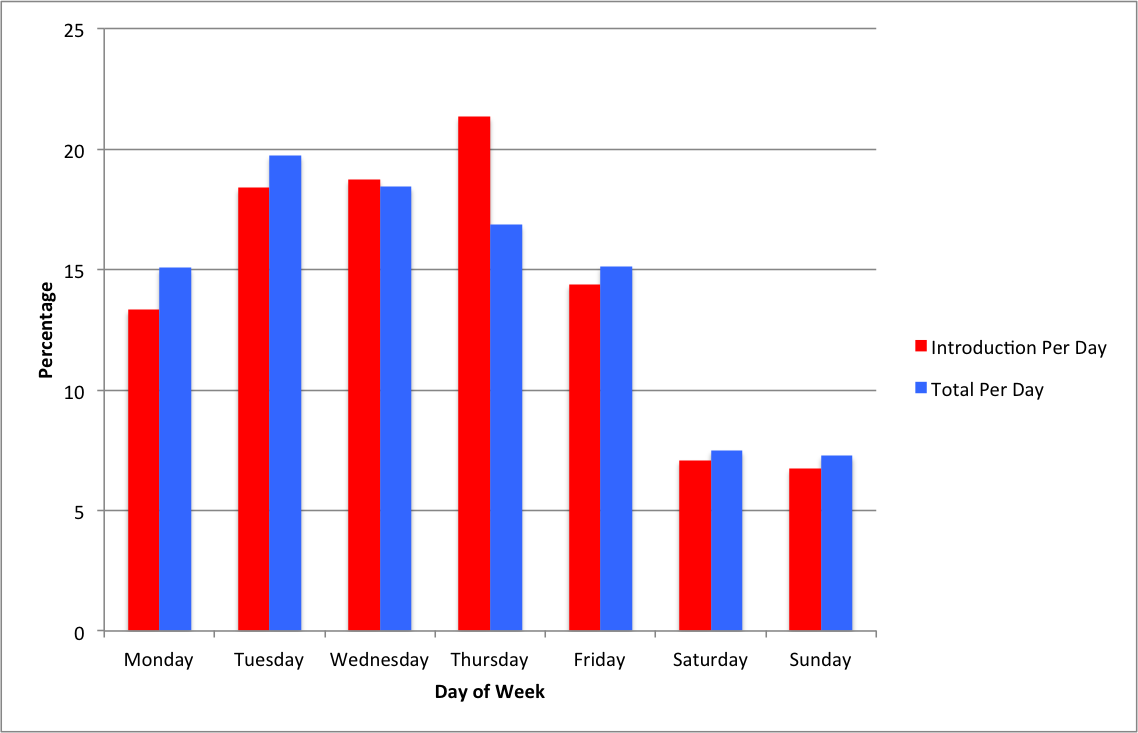
\includegraphics[width=0.6\textwidth]{firefox_bug_introduction_day_of_week.png}
\end{center}
\caption{Firefox percentage of bug introductions and percentage of total commits per day}
\label{fig-firefox-weekday}
\end{figure*}

First we determine if the day of the week has any impact on the
likelihood of producing bugs. For the following graphs the percentage
of introduction commits indicates the amount of commits out of the
total number of commits which are bug introductions. Our results from
Linux are shown in Figure \ref{fig-linux-weekday}. We see that
Saturday is the worst day followed by Thursday, while Monday has the
fewest percentage of bug introductions. The results for Firefox are
shown in Figure \ref{fig-firefox-weekday} and agree with Thursday
being one of the worse days while Monday is the best for committing
changes which do not introduce bugs. A possible explanation is that
developers rest over the weekend and have ample time to think about
the problem before writing it on Monday when they know exactly what to
do. It may also be correlated to the size of the change which we plan
to investigate later as an addition to our technique.

\begin{figure*}
\begin{center}
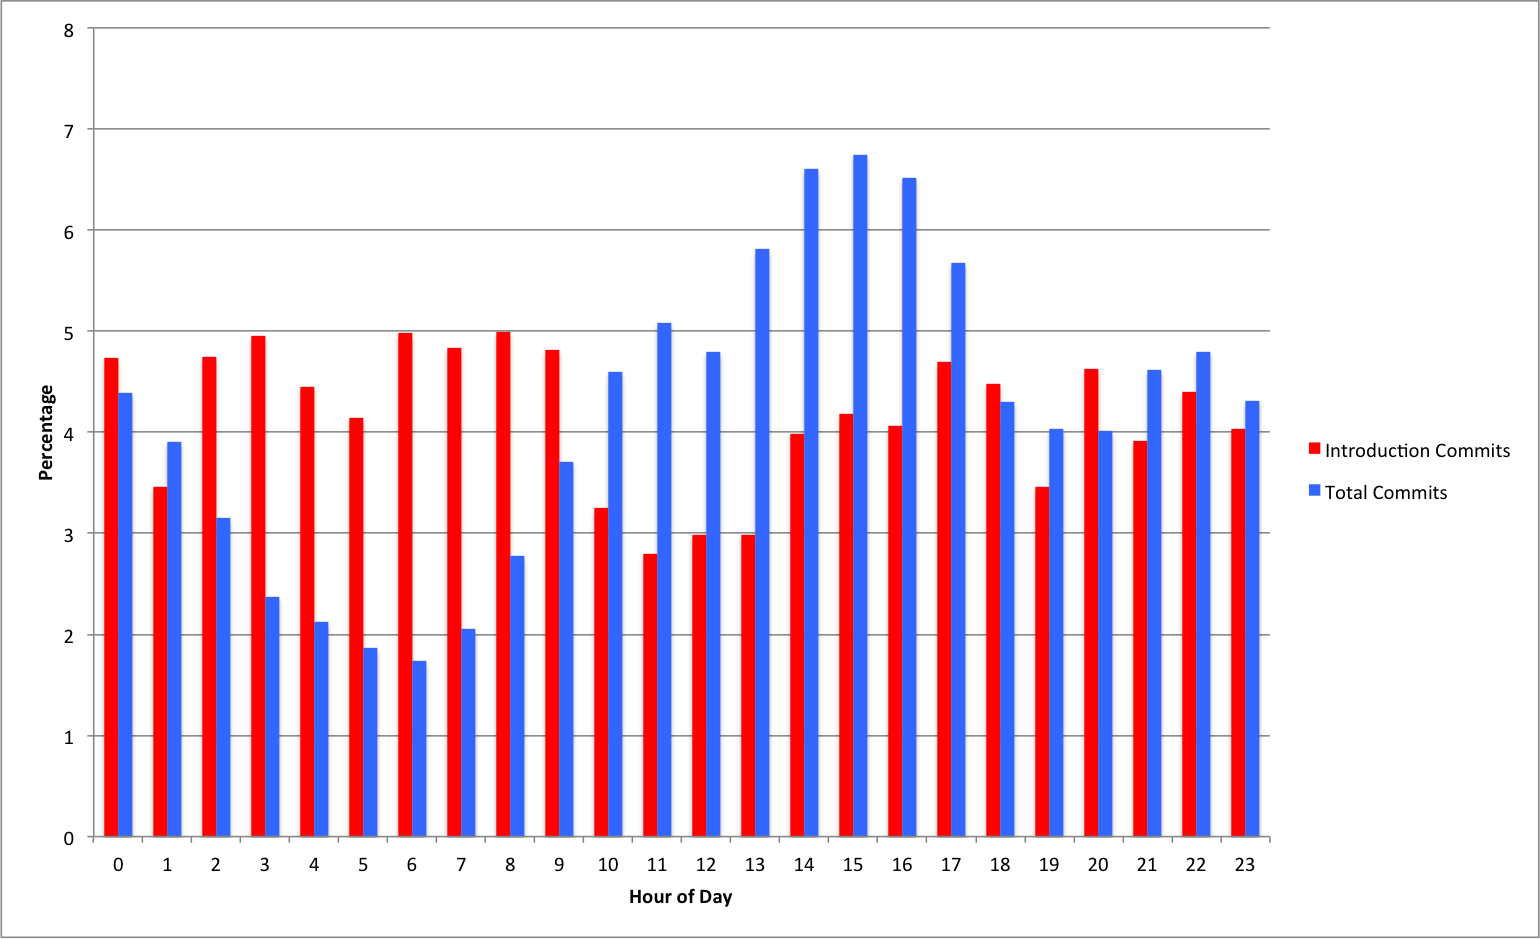
\includegraphics[width=0.9\textwidth]{linux_hour_of_day.png}
\end{center}
\caption{Linux percentage of bug introductions and percentage of total commits per hour}
\label{fig-linux-hour}
\end{figure*}

\begin{figure*}
\begin{center}
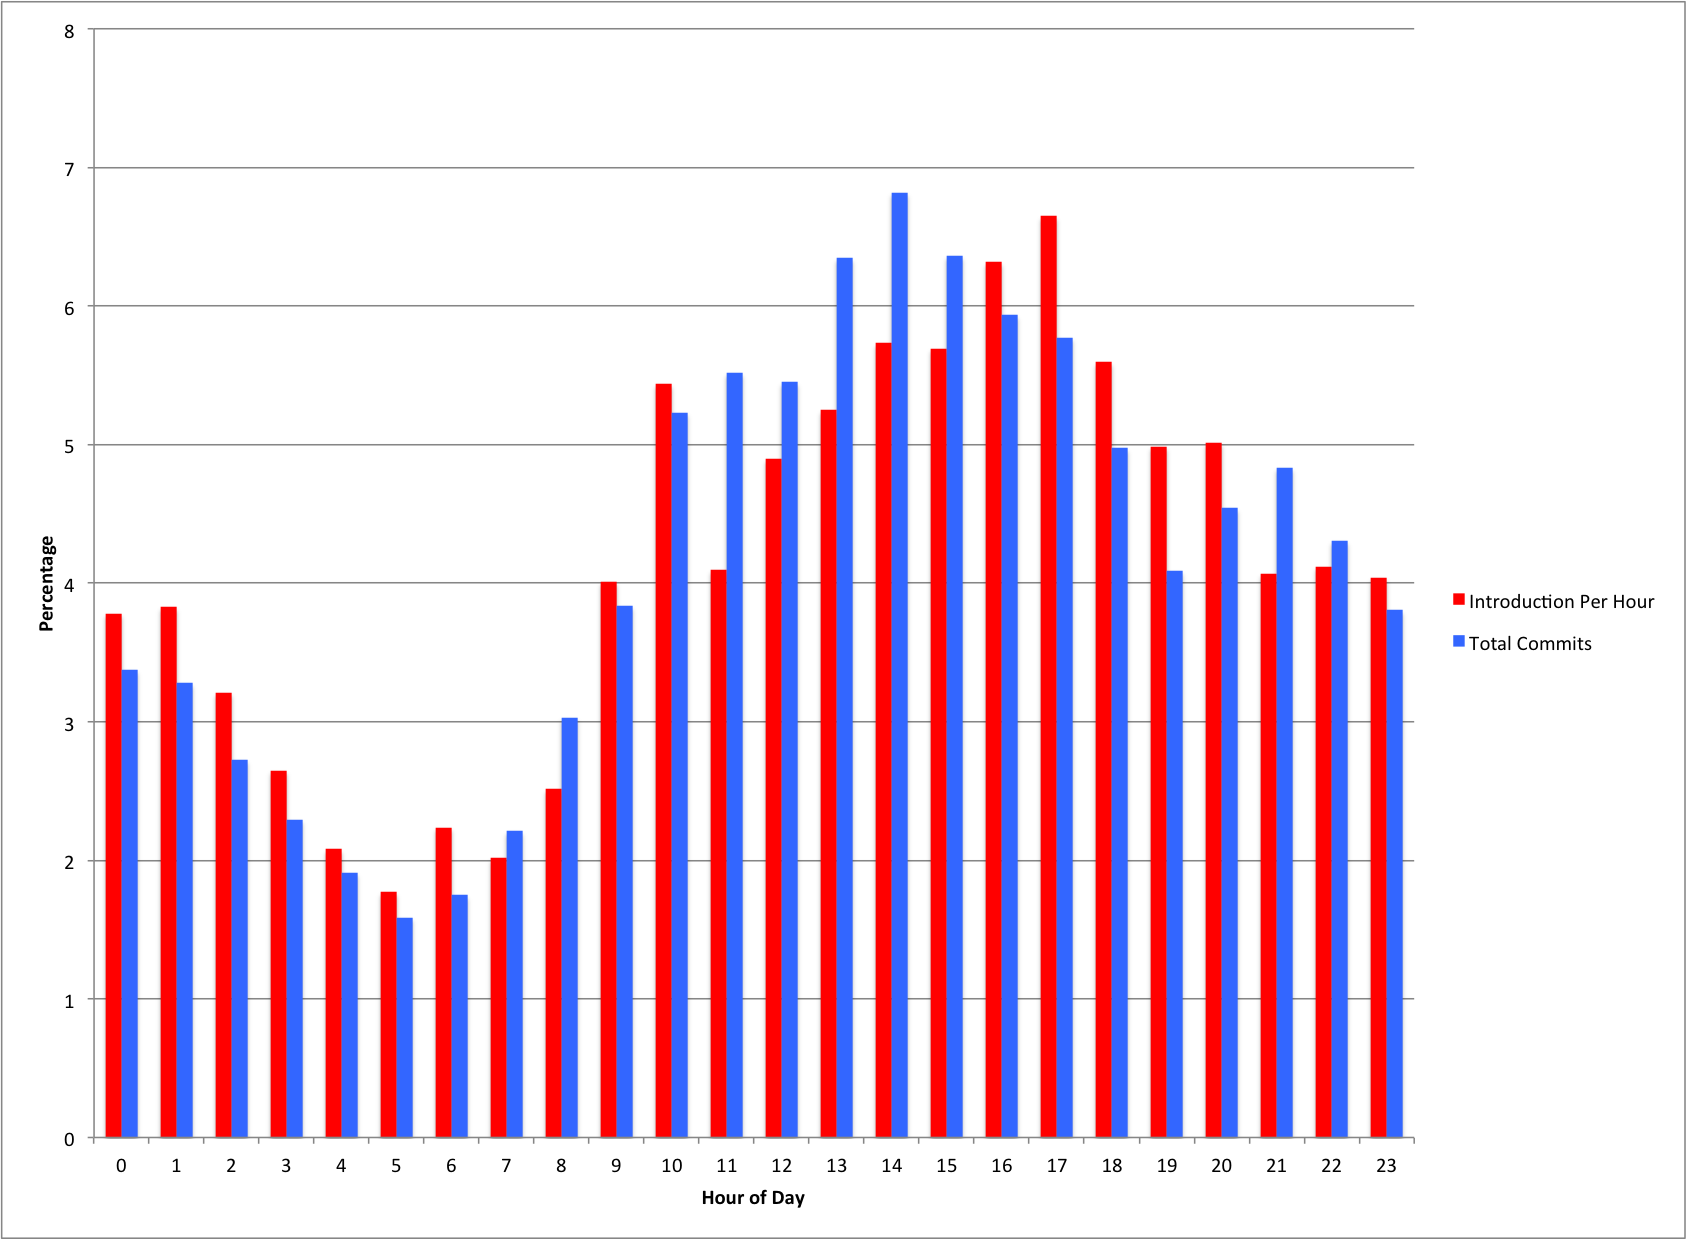
\includegraphics[width=0.9\textwidth]{firefox_hour_of_day.png}
\end{center}
\caption{Firefox percentage of bug introductions and percentage of total commits per hour}
\label{fig-firefox-hour}
\end{figure*}

Next we determine if the hour has any impact. Our results from Linux
and Firefox are shown in Figure \ref{fig-linux-hour} and Figure
\ref{fig-firefox-hour} respectfully. Both show a significant increase
in the amount of commits which introduce a bug between midnight and 9
AM. After this time there is a significant reduction in the amount of
bug introductions between 11 AM and 3 PM. After 3 PM however, the
likelihood of bug introductions fluctuates from hour to hour. This
result is not very surprising since tired programmers are more likely to
produce mistakes. It does however indicate the hours that programmers
are at the peak of their productiveness in terms of not creating
additional bugs.

\begin{figure*}
\begin{center}
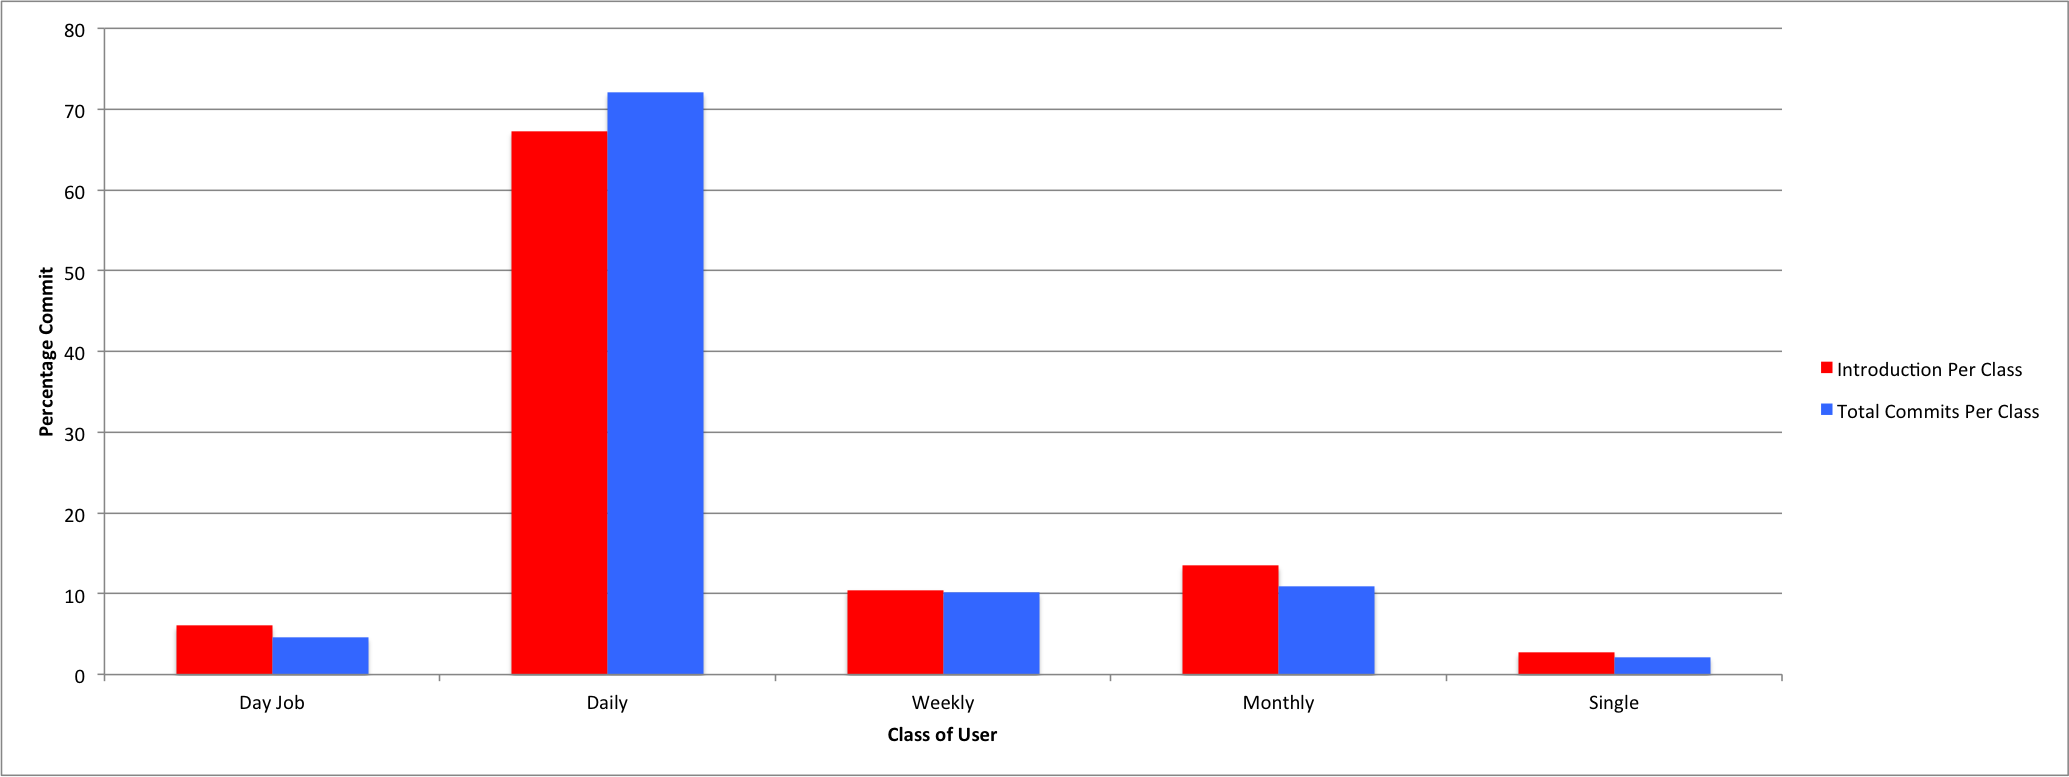
\includegraphics[width=0.9\textwidth]{linux_per_class.png}
\end{center}
\caption{Linux percentage of bug introductions and percentage of total commits per author classification}
\label{fig-linux-class}
\end{figure*}

\begin{figure*}
\begin{center}
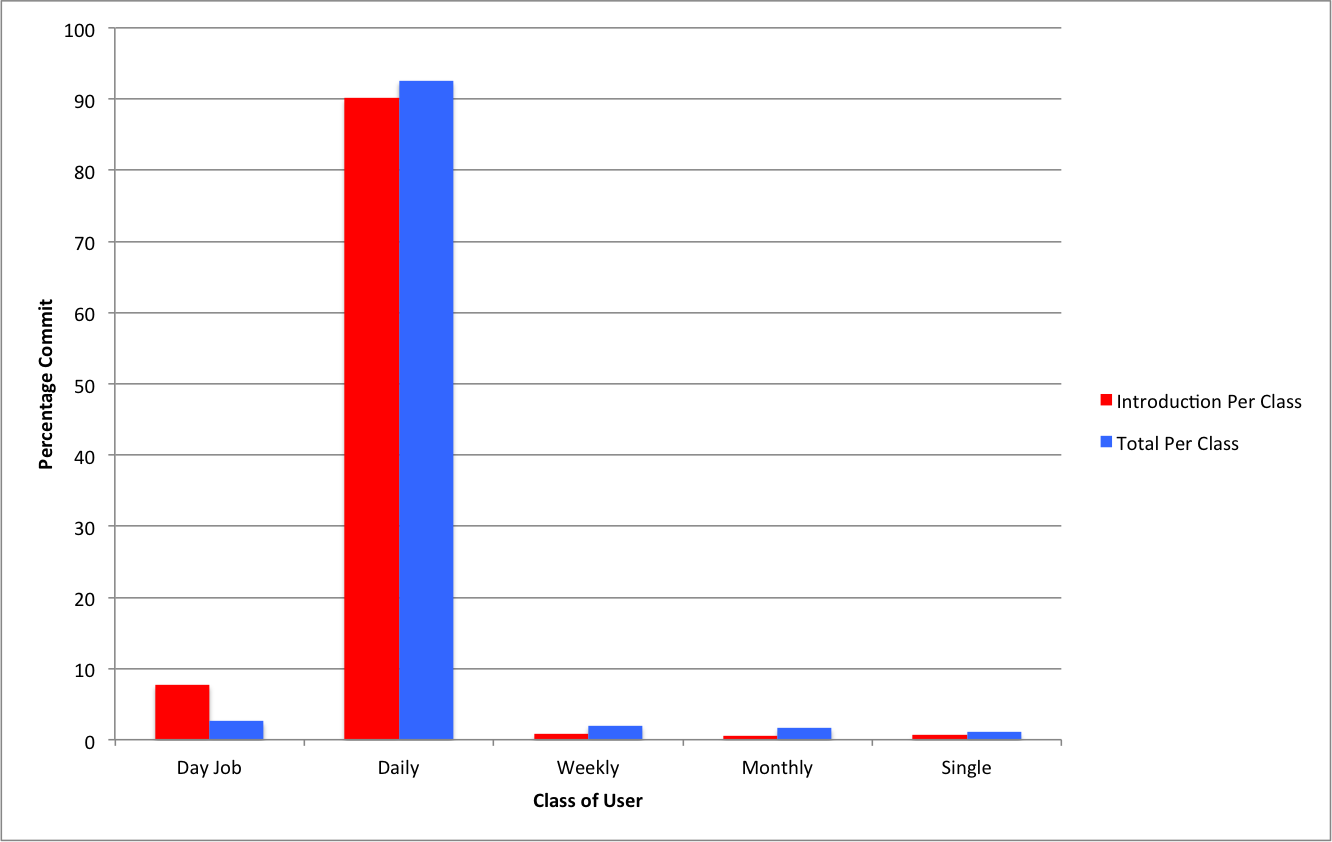
\includegraphics[width=0.6\textwidth]{firefox_per_class.png}
\end{center}
\caption{Firefox percentage of bug introductions and percentage of total commits per author classification}
\label{fig-firefox-class}
\end{figure*}

We then investigated how each classification of developers fair in
terms of their likelihood of creating a bug. The results from Linux
and Firefox are shown in Figure \ref{fig-linux-class} and Figure
\ref{fig-firefox-class} respectfully. We see that developers who
commit changes daily are a very significant portion of both projects
and not developers that work on code as part of their day job. This
trend is likely to be common to most open source projects. We also see
for both projects the daily developers are less likely to produce
bugs. On the other hand developers with this as their day job are more
likely to produce bugs. The cause of this could be that the developers
with this as their day job are required to make changes, while the
daily developers are motivated purely by interest.

\begin{figure*}
\begin{center}
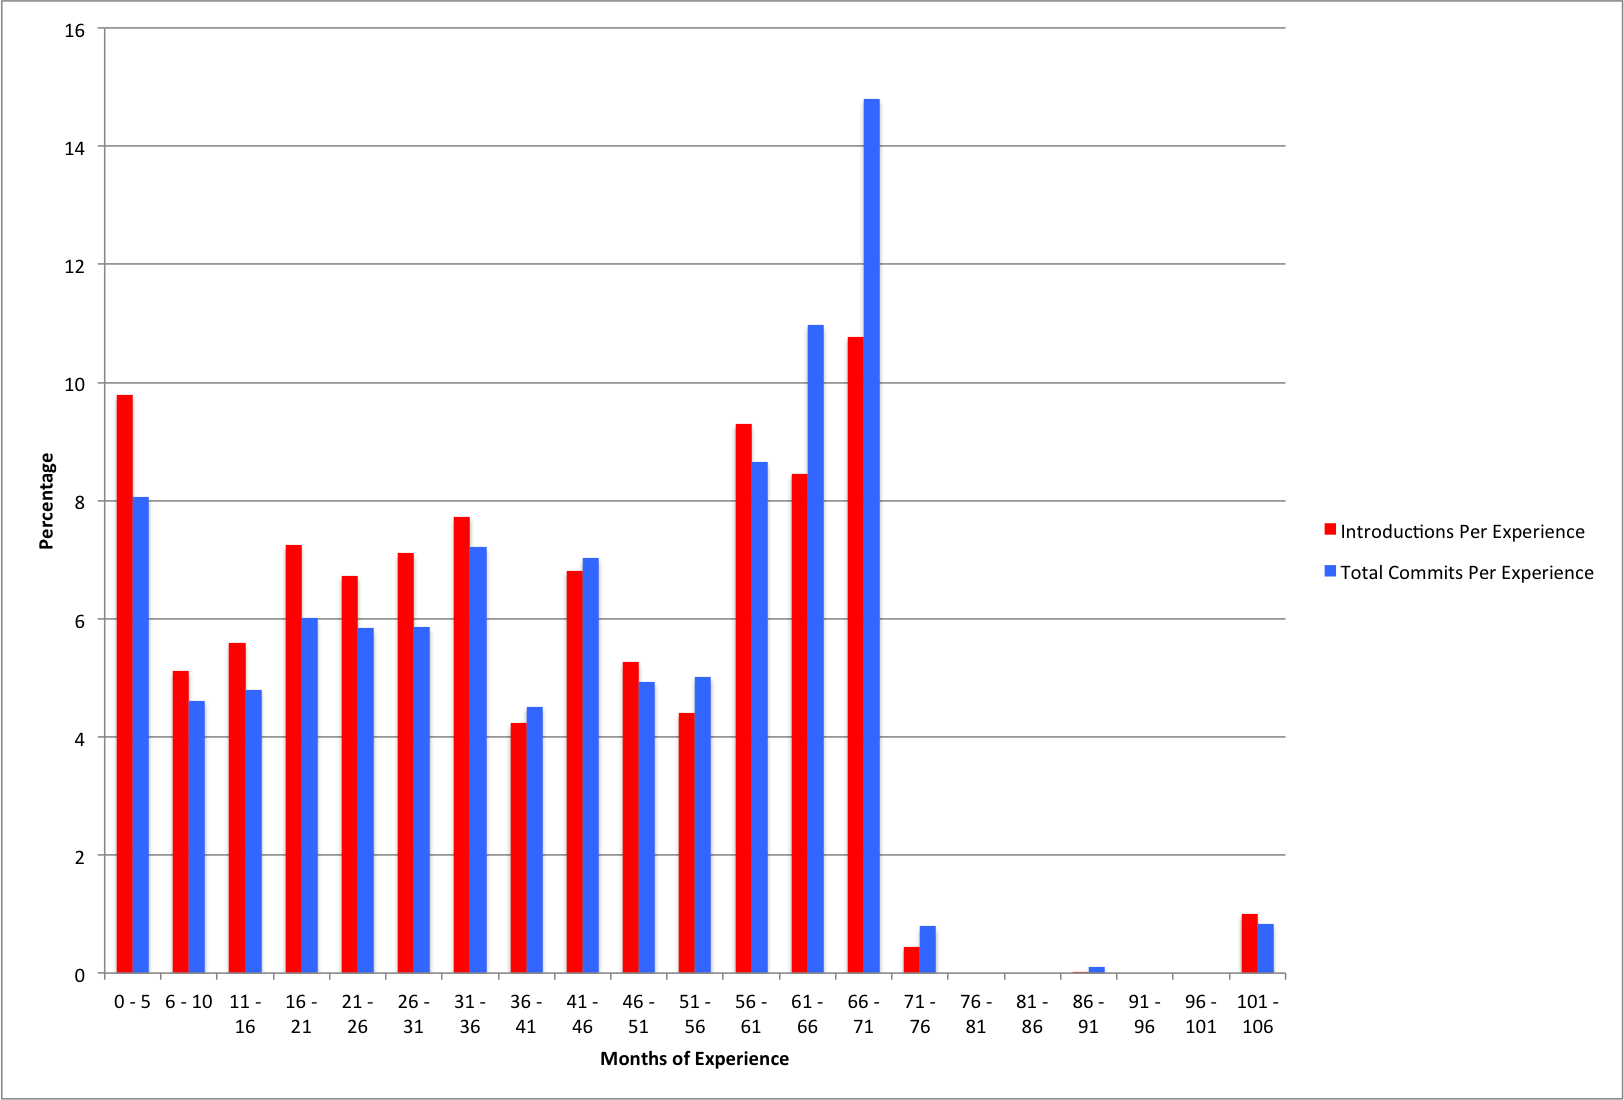
\includegraphics[width=0.9\textwidth]{linux_day_per_experience.png}
\end{center}
\caption{Linux percentage of bug introductions and percentage of total commits per author experience}
\label{fig-linux-experience}
\end{figure*}

\begin{figure*}
\begin{center}
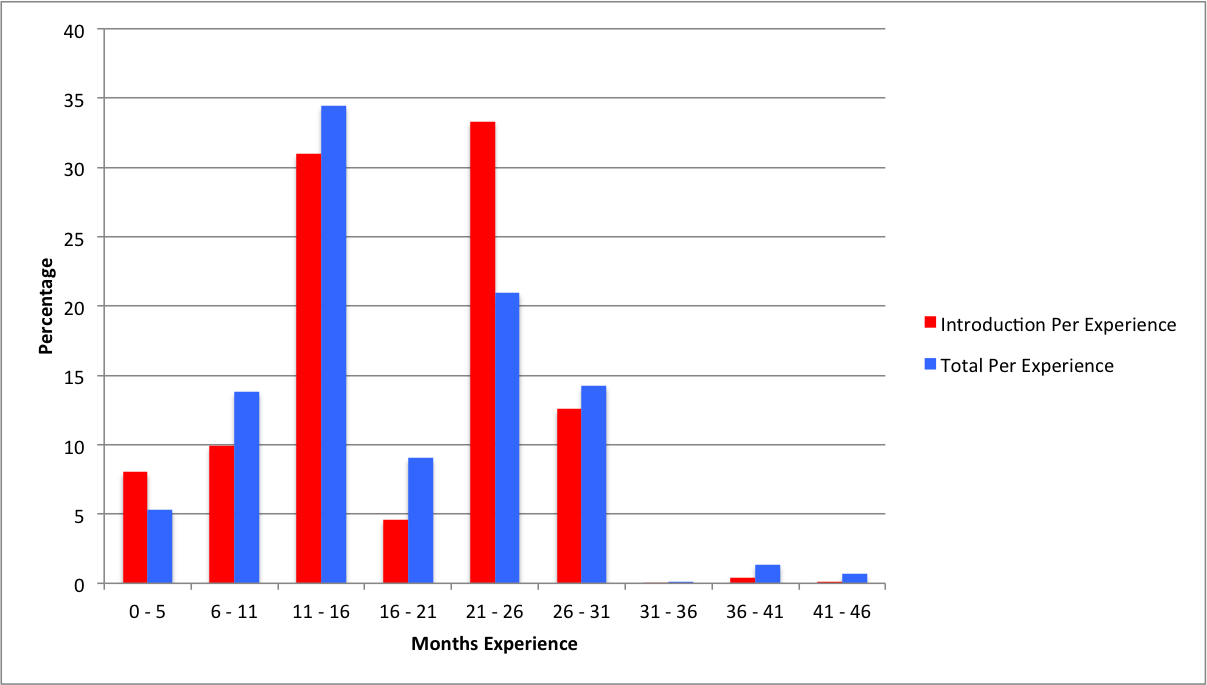
\includegraphics[width=0.6\textwidth]{firefox_day_per_experience.png}
\end{center}
\caption{Firefox percentage of bug introductions and percentage of total commits per author experience}
\label{fig-firefox-experience}
\end{figure*}

The final head-to-head comparison we performed is based on the amount
of experience per author. We divided them up into 6 months intervals. 
Our results from Linux and Firefox are shown in Figure
\ref{fig-linux-experience} and Figure \ref{fig-firefox-experience}
respectfully. For Linux authors with less than 2 years of experience
are more likely to commit a bug while after 2 years the likelihood
decreases. However the authors which committed throughout the history
of the project are more likely to commit a bug which may be because
they wrote the majority of the code. For Firefox, again the
developers with less than 6 months of experience are more likely to
commit a bug. The is a spike between 21 and 26 months as well. We
believe these results may not be accurate due to the possiblity of
our experience metric being crude and not representative of the 
actual experience with the project.

\begin{figure*}
\begin{center}
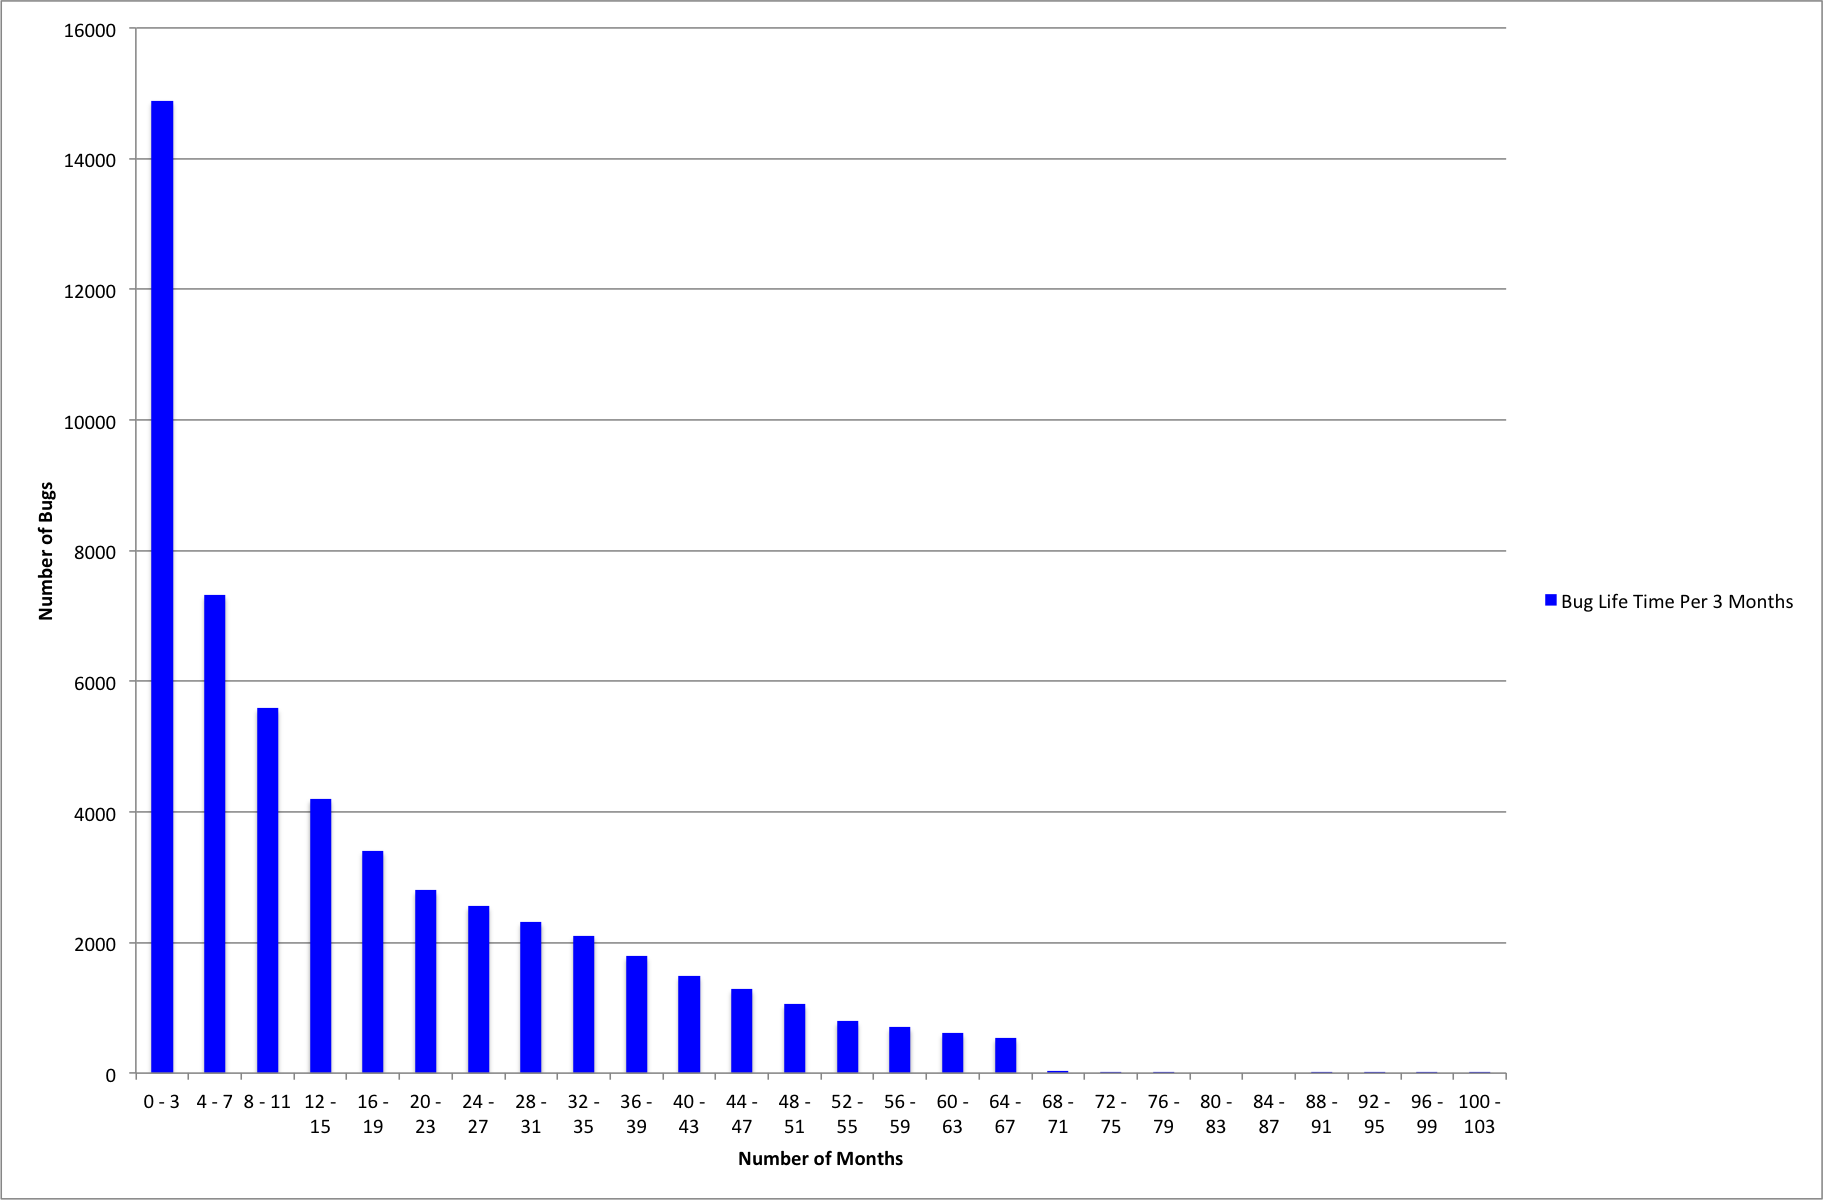
\includegraphics[width=0.9\textwidth]{linux_bug_life.png}
\end{center}
\caption{Linux number of bugs against bug lifetimes in months}
\label{fig-linux-buglife}
\end{figure*}

\begin{figure*}
\begin{center}
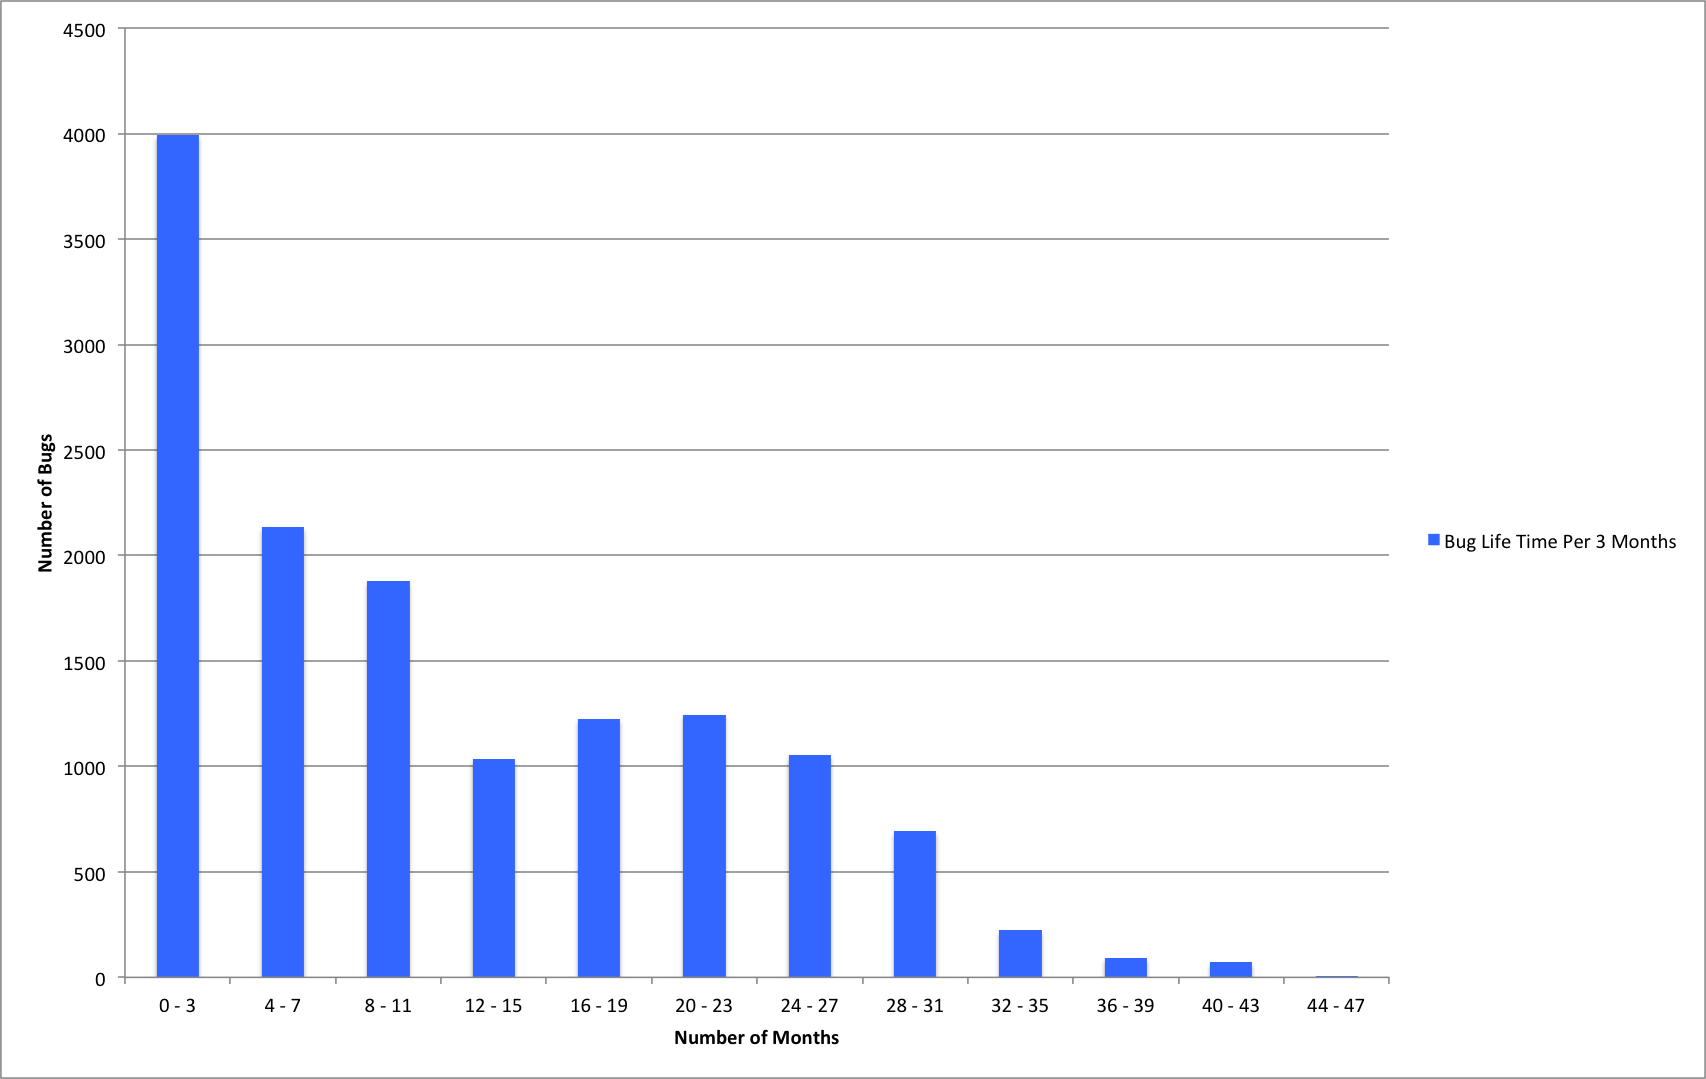
\includegraphics[width=0.9\textwidth]{firefox_bug_life.png}
\end{center}
\caption{Firefox number of bugs against bug lifetimes in months}
\label{fig-firefox-buglife}
\end{figure*}

Finally we determined the bug lifetimes for both projects to contrast
them to previous work. We plotted the number of bugs for each lifetime
divided into 4 month intervals. The results for Linux are shown in
Figure \ref{fig-linux-buglife}, the average bug lifetime is 1.39
years. The results for Firefox are shown in Figure
\ref{fig-firefox-buglife}, with an average bug lifetime of 0.97
years. This shows a reduction in the average bug lifetime for Linux (in
2002 the average lifetime was 1.8 years). This indicates that
developers are improving as their development process becomes more
refined. We also see the average lifetime is lower for Firefox, this
may be due to the complexity of the software, size of the software or
the amount of users (the more users and complex, the more likely bugs will be
revealed).


